%%%%%%%%%%%%%%%%%%%%%%%%%%%%%%%%%%%%%%%%%%%%%%%%%%%%%%%%%%%%%%%%%%%%%%%%%%%%
%% Trim Size : 11in x 8.5in
%% Text Area : 9.6in (include Runningheads) x 7in
%% ws-jai.tex, 26 April 2012
%% Tex file to use with ws-jai.cls written in Latex2E.
%% The content, structure, format and layout of this style file is the
%% property of World Scientific Publishing Co. Pte. Ltd.
%%%%%%%%%%%%%%%%%%%%%%%%%%%%%%%%%%%%%%%%%%%%%%%%%%%%%%%%%%%%%%%%%%%%%%%%%%%%
%%

%\documentclass[draft]{ws-jai}
\documentclass{ws-jai}
\usepackage[flushleft]{threeparttable}
\usepackage{pdflscape}
\usepackage{longtable} 
\def\btex{B{\sc IB}\TeX\ }
\begin{document}

\catchline{}{}{}{}{} % Publisher's Area please ignore

\markboth{Jack Hickish, CASPER gang, etc.}{The Collaboration for Astronomy Signal Processing and Electronics Research in 2016.}

\title{The Collaboration for Astronomy Signal Processing and Electronics Research in 2016}

%\author{First Author$^\dagger$, Second Author$^\ddagger$, Third Author$^\ddagger$ and Fourth Author$^\S$}
\author{Jack Hickish$^\dagger$, Others$^\ddagger$}

\address{
$^\dagger$Radio Astronomy Laboratory, UC Berkeley, Berkeley, CA 94720, USA, jackh@astro.berkeley.edu\\
$^\ddagger$Group, Company, Address, City, State ZIP/Zone, Country\\
$^\S$Group, Company, Address, City, State ZIP/Zone, Country, fauthor@company.com
}

\maketitle

\corres{$^\dagger$Jack Hickish}

\begin{history}
\received{(to be inserted by publisher)};
\revised{(to be inserted by publisher)};
\accepted{(to be inserted by publisher)};
\end{history}

\begin{abstract}

The Collaboration for Astronomy Signal Processing and Electronics Research
(CASPER) has been working for a decade to reduce the time and cost of designing,
building and deploying new digital radio astronomy instruments.  Today,
CASPER-designed hardware powers some ?? scientific instruments worldwide, and
are used by scientists and engineers at ?? academic institutions.  In this paper
we summarize the current offerings of the CASPER collaboration, focussing on
currently-available and next-generation hardware.  We describe the ongoing state
of software development, as CASPER looks to support an ever-increasing selection
of off-the-shelf digital signal processing platforms.

\end{abstract}

\keywords{CASPER, digital signal processing, radio astronomy, instrumentation}

\section{Introduction}

Since the first digital instrument used in radio astronomy \citep{Weinreb} we
have seen a growing adoption of digital processing hardware as the foundation on
which radio telescopes are built.  Today, CPUs, GPUs, FPGAs and ASICs power
almost all of the world's radio telescopes, and our ability to do science has
become inextricably linked with our ability to perform digital computation.
With the capability of digital processing hardware scaling exponentially with
Moore's law, the ability to leverage current technology by reducing the
design-time of new instruments is critical in effective deployments of new radio
astronomy instruments.

The Collaboration for Astronomy Signal Processing and Electronics Research
(CASPER) puts \emph{time-to-science}, the time between conception of an
instrument and its deployment, as a central figure of merit in instrument
design. CASPER works to minimize time-to-science by working to develop and
support open-source, general-purpose hardware, software libraries and
programming tools which allow rapid instrument design, and straightforward
upgrade cycles.

With CASPER hardware and software now powering some ?? radio astronomy
instruments worldwide (see Table~\ref{table:casper-instruments}) including some
of the largest, most advanced telescopes ever built, such as the upcoming
MeerKat Array\footnote{\url{http://public.ska.ac.za/meerkat/meerkat-schedule}}, it is appropriate to document the state of the
Collaboration.

In this paper, we first summarize the design philosophy of CASPER in
Section~\ref{sec:CASPER-philosophy}.  In Section~\ref{sec:Hardware} we describe
currently available CASPER hardware offerings, including the range of digitizers
developed and supported by CASPER. Key to CASPER's success are the firmware
libraries and programming infrastructure provided by the collaboration, which we
overview in Section~\ref{sec:Software}.  In Section~\ref{sec:Deployments} we
document the extensive and wide-ranging applications to which CASPER hardware
and design-tools have been applied. Finally, we describe the future direction of
and challenges faced by the CASPER collaboration in Section~\ref{sec:Future},
with concluding remarks in Section~\ref{sec:Conclusions}.

\section{The CASPER Philosophy} \label{sec:CASPER-philosophy}

%% Jason Manley's PHD has a good section on Philosophy and Ethernet.
World-wide, radio astronomy is a relatively small industry and has minimal financial incentive attracting investors. This means that often institutions often rely heavily on government funding. It is therefore beneficial to share resources between organisations as to leverage the work that others have put into developing radio astronomy instrumentation. For this reason institutions often open source their intellectual property. CASPER was founded to aid this collaboration. It aims to share and collaborate on both hardware and software for the design of radio astronomy DSP systems.

The CASPER community has designed multiple FPGA based hardware platforms and the software tools to design and support these platforms.

Along with hardware platforms, CASPER provides a tool-flow based on the Matlab, Simulink and Xilinx System Generator (XSG) tools to enable a designer to easily design and target a particular hardware platform \cite{pars05}. The interface is a graphical design environment in Simulink where a designer can drag and drop blocks and connect them with wires in the desired configuration. A library of CASPER Digital Signal Processing (DSP) blocks are provided. These are targeted at the particular type of DSP typical of radio astronomy data processing. In addition, there is also a library of hardware specific blocks, which contain the controllers for ADCs and Ten Gigabit Ethernet (TGE) modules, amongst others. The flow provides a "One-Click" solution from design to bitstream, ready to upload onto a board. The DSP parts of the design are easily transferable to other Xilinx FPGA hardware. This eases upgrades to new hardware, as well as aiding collaboration between teams using different CASPER hardware platforms \cite{pars05}. 

CASPER makes use of Ethernet as a generic backplane architecture, to provide packetised interconnects between hardware modules. In this way, instruments can consist of different types of data processing hardware. For example, it is easy to hand off parts of the processing chain to a GPU cluster by redirecting the data sent over the network to different Internet Protocol (IP) address. A design can even leverage the IP Multicast protocol\footnote{IP multicast is described in RFC 1112} which allows additional instruments to subscribe to the data and process it concurrently alongside the main instrument. This keeps the problem of full cross-bar interconnects in the domain of the switch manufactures and allows instrument designers to focus on digital signal processing \cite{man14}, \cite{pars05}.

Overall, CASPER has a progressive philosophy towards instrumentation design and it is important to take into account when examining, designing and implementing tools to be used by this community and others.

\subsection{Computing by the yard}

\subsection{Ethernet}

\subsubsection{Multicast \& Commensal Instruments}


\section{CASPER Hardware} \label{sec:Hardware}

Since its inception, the collaboration has produced a range of hardware with particular focus on FPGA boards and supporting hardware such as Analog-to-Digital Converters (ADC) and Ethernet mezzanine cards. 

\subsection{FPGA platforms}

Much of the focus of the community has moved from the popular ROACH2 platform to the newer SNAP and SKARAB boards which sport the Xilinx Kintex and Virtex FPGAs, respectively. This section, therefore, will focus on the SKARAB and SNAP hardware platforms.

\subsubsection{ROACH1}

For completeness it is important to mention the grandfather of the current hardware generation, the ROACH1. The architecture is based on a single FPGA with a control processor and mezzanine connectors for the addition of ADCs and other peripherals \cite{Casp09}. The core of the ROACH is the Xilinx Virtex 5 xc5vlx110t chip. The CASPER tools still provide support for this board even though it is two generations old.

%% Wesley New

\subsubsection{ROACH2}

The ROACH2 is the update to the ROACH platform, the major differences being the Xilinx Virtex 6 FPGA and the addition of two mezzanine slots which could be used for memory or Ethernet cards \cite{Casp12}.
%% Wesley New

\subsubsection{SKARAB}

The Square Kilometre Array Reconfigurable Application Board (SKARAB) hardware is the next generation FPGA hardware platform that has been designed by a South African company, Peralex, according to the specifications of SKA-SA, as an alternative to the ROACH2 hardware for applications requiring better processing performance. The departure from the ``ROACH'' naming convention to the ``SKARAB'' naming convention is because the interfaces between the ROACH2 and the SKARAB are not compatible.

A functional block diagram of the SKARAB is presented in Figure~\ref{fig:skarab_bd} \cite{cliff16}.

\begin{figure}[h]
\centering
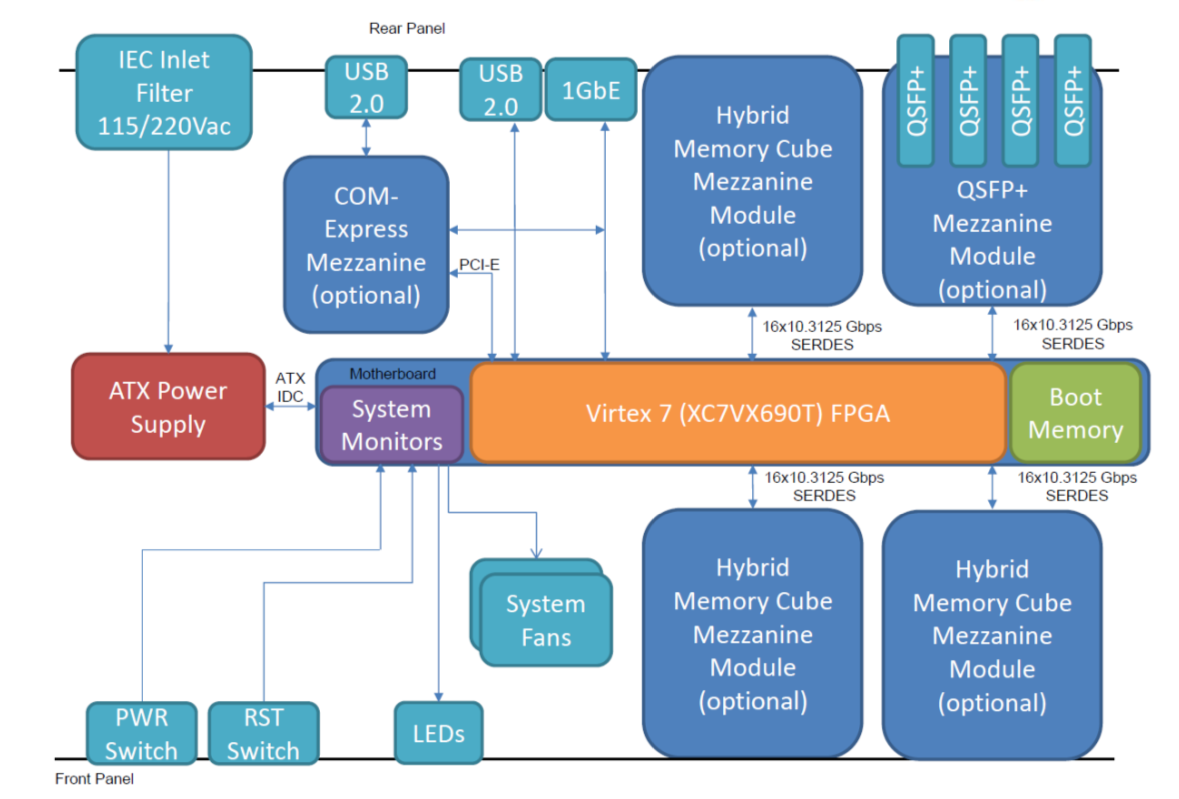
\includegraphics[width=150mm, scale=0.5]{skarab_bd}
\caption{SKARAB Functional Block Diagram}
\label{fig:skarab_bd}
\end{figure}

At the heart of the SKARAB processing, lies the Xilinx Virtex 7 FPGA (XC7VX690T). This FPGA consists of 693120 logic cells, 52 Mb of internal random access memory (RAM) blocks and 3600 digital signal processing (DSP) slices \cite{cliff16}. Nearly all of the input/output (I/O) available is high-speed serial/deserializer (SERDES) I/O \cite{Teag15}. 

The SKARAB makes provision for four mezzanine sites with each site interfacing with sixteen transmit and sixteen receive 10 Gbps SERDES lines \cite{cliff16}. This means each site can handle a throughput of 160 Gbps and if all the sites are utilized, a total of 640 Gbps can be achieved.

There is no power personal computer (PPC), but provision has been made for the COM Express mezzanine site which can interface with an external processor via single lane PCIe \cite{Teag15}.
 
The SKARAB has already been tested with two existing mezzanine cards: QSFP+ Mezzanine Module and the Hybrid Memory Cube (HMC) Mezzanine Module. The Peralex QSFP+ Mezzanine Module supports four 40Gb Ethernet interfaces and the SKA-SA HMC Mezzanine module provides external memory storage for the processing using high speed serial memory \cite{cliff16}.     

The hardware of the SKARAB is presented in Figure~\ref{fig:skarab_hw} \cite{cliff16}.

\begin{figure}[h]
\centering
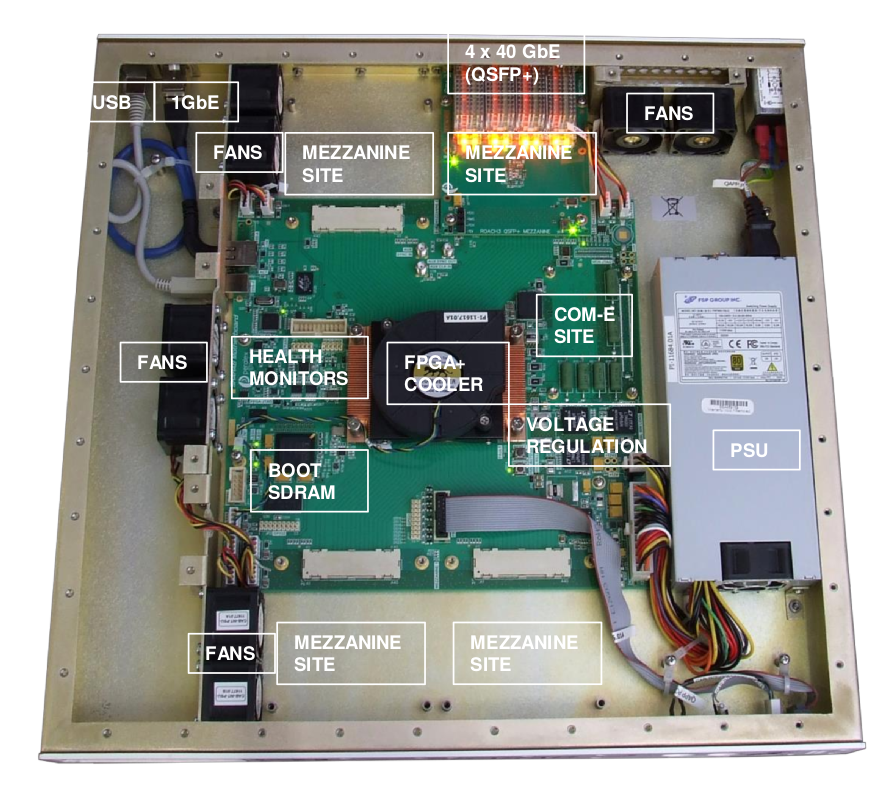
\includegraphics[width=150mm, scale=0.5]{skarab_hw}
\caption{SKARAB Hardware}
\label{fig:skarab_hw}
\end{figure}

The SKARAB board support package (BSP) comes with the 40GbE core, 1GbE core, HMC core and the management microcontroller, which runs on the FPGA (Xilinx's microblaze processor) \cite{cliff16}. The management microcontroller sets up the network (1GbE, 40GbE), performs FPGA configuration (1GbE), monitors the voltages and currents, monitors and controls the fan speeds and handles communication to/from the FPGA via the wishbone bus \cite{cliff16} \cite{Teagu15}.
 
The SKARAB BSP is currently being added to the CASPER tool flow and should be ready in December 2016.
SKA-SA will be integrating 300 SKARAB units, as part of the MeerKAT upgrades, and should be ready for operation latest by the end of 2017.

%% Adam Isaacson

\subsubsection{SNAP}

\subsection{ADCs \& DACs}

% NOTE: I just took the list from the website, are there others, are these all legit? (Griffin)
\begin{tabular}{lccccc}
Name & Type & Bits & Sample Rate & Inputs/Outputs & Interface \\
\hline
ADC2x1000-8 (iADC) & ADC & 8 & 1 GSPS & 2 & Z-DOK \\
ADC1x3000-8 & ADC & 8 & 3 GSPS & 1 & Z-DOK \\
ADC64x64-12 & ADC & 12 & 64 MSPS & 64 & Z-DOK x2 \\
ADC4x250-8 (QuADC) & ADC & 8 & 250 MSPS & 4 & Z-DOK \\
ADC2x550-12 & ADC & 12 & 550 MSPS & 2 & Z-DOK \\
ADC2x400-14 & ADC & 14 & 400 MSPS & 2 & Z-DOK \\
KatADC & ADC & 8 & 1.5 GSPS/3.0 GSPS & 2/1 & Z-DOK \\
ADC1x5000-8 & ADC & 8 & 5 GSPS & 1 & Z-DOK \\
ADC16x250-8 & ADC & 8 & 1 GSPS/500 MSPS/250 MSPS & 4/8/16 & Z-DOK \\
ADC1x10000-4 & ADC & 4 & 10 GSPS & 1 & Z-DOK \\
DAC2x1000-16 & DAC & 16 & 1 GSPS & 2 & Z-DOK \\
\end{tabular}

\section{CASPER Software \& Programming Tools} \label{sec:Software}

\subsection{The CASPER Tool Flow}

%% Wesley New

\subsection{JASPER Tool Flow}

%% Jack Hickish to introduce this and explain history

%% Adam Isaacson to explain the latest additions
The JASPER tool flow is currently being upgraded to make provision for additional front ends and back ends besides Simulink and Xilinx, respectively. This will prevent the developer from being tied down to a specific software package and FPGA platform \cite{Isaac16}. The current upgrades are presented in Figure~\ref{fig:jasper_ug_bd} \cite{Isaac16}.

\begin{figure}[h]
\centering
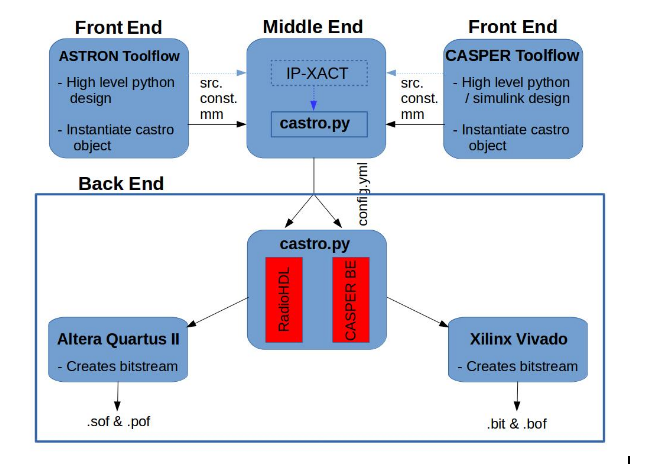
\includegraphics[width=150mm, scale=0.5]{jasper_ug_bd}
\caption{JASPER Upgrade Tool Flow Diagram}
\label{fig:jasper_ug_bd}
\end{figure}  

The Front-End includes the structural VHDL or any modelling tools e.g. Matlab/Simulink, Labview, Sci-Lab/Sci-Cos and MyHDL. It includes a script which will instantiate the python classes inside the Middle End process \cite{Isaac16}. 

The python classes are located in the Middle End (castro.py) file. In the future, it is likely that the Front End will come in through another interface e.g. possibly IP-XACT in order to make provision to interface to other simulation tools e.g. Sci-Cos and Sci-Lab. This interface is denoted by the dashed lines in Figure~\ref{fig:jasper_ug_bd}. IP-XACT is an IEEE standard and is used to integrate different IP packages together, provided that the IP interfacing meets the IP-XACT standard. The IP-XACT interface would be in the form of an XML script. The decision to utilise IP-XACT has not been finalised yet. The castro.py is passed all the Front End memory map, constraints and source files. The castro.py script takes this metadata from the Front End and dumps all of this metadata into a YAML configuration file (config.yml). It should be noted that the Middle End module is not platform agnostic due to the hardware and platform metadata \cite{Isaac16}.

The Back End consists of the same castro python class that exists in the Middle End. The castro.py python script will load the config.yml file/metadata and instantiate python objects with this metadata, which will either be sent to RadioHDL if targeting the Altera hardware or the Casper Back End, if targeting the Xilinx hardware. This will also allow the user to target other vendor hardware in the future e.g. Lattice and Actel and due to the common castro.py python script, it will easier to just add an additional back end \cite{Isaac16}. 

The RadioHDL process will then generate the necessary Quartus project files and run the compiler. The output of the process will be the Altera FPGA SRAM Object file (sof) and Programming Object File (pof). The Casper Back End generates the necessary tcl scripts, which runs the Vivado compiler. The output of the process is the Xilinx FPGA bit and Borph Object File (bof) programmable files \cite{Isaac16}.

The current release of the JASPER tool flow actually includes the castro python class and the CASPER back end makes provision for both Xilinx ISE and Vivado. The JASPER tool flow also makes provision for the SKARAB platform and the generation of the fpg configuration files, which are used for the ROACH2 and SKARAB configuration \cite{Balla16}.

%% Adam Isaacson / Jack Hickish

\subsection{CASPER DSP Libraries}

%% Andrew Martens + anyone else keen to contribute

% NOTE: First draft of section, please feel free to edit (Griffin)
% TODO: add CBASS-south, AVN Ghana, KuPol to instrument list

In order to quickly and easily develop new radio astronomy instruments a number
of DSP blocks have been developed for use in CASPER board firmware. Typical
instruments such as spectrometers, beamformers, correlators, ADC recorders, and
DAC signal generators are constructed from this library of DSP blocks.

These blocks are based on the low-level logical units provided by the Xilinx
Simulink library and the generic Simulink libraries. Configurable low-level DSP
blocks are then used to build more complex, high-level DSP blocks. This
heirarchical design style enables quick and uniform logic development through
block reuse. High-level blocks include configuration parameters which are
propagated through the low-level logic to update the underlying logic. Thus,
generic blocks such as streaming FFTs and vector accumulators are included in
the library, and configured when placed into a firmware design.

Matlab Simulink provides a 2-D, heirarchical design and simulation environment
useful for firmware design. Individual DSP blocks are placed into a model
design, and connected via data lines. Once a firmware model has been laid out
test vectors can be simulated through the system to verify the logic with a test
bench.

Xilinx provides the basic libraries to build firmware for their FPGAs. Basic
blocks include logic gates, multipliers, adders, signal delays, FIFO buffers and
block RAM (BRAM) interfaces. Blocks in the CASPER library are written using
these basis blocks. Blocks can also be wrappers for HDL code, such as with the
external interfaces. A number of specialized basic blocks have been written in
the CASPER library for radio astronomy applications. For example, many low-bit
complex multipliers are often used in correlation, to improve the resource
efficiency a specialized 4-bit multiplier has been written. Also typical in
firmware design is signal reorders and transposes, general blocks have been
written to facilitate ease of BRAM memory use for these operations.
Documentation on the CASPER library can be found
online\footnote{https://casper.berkeley.edu/wiki/Block\_Documentation}.

Using these basic logic and memory building blocks more complex DSP modules have
been developed. At the core of many radio astronomy instruments is a fast Fourier
Transform operation. A generic FFT module is implemented using a radix-2,
biplex, decimation-in-time design. This module computes the Fourier Transform on
a window of $2^N$ complex samples and is highly configurable. An efficient
real-input FFT and a multi-input 'wideband' FFT module have been implemented
using the generic FFT. In order reduce FFT sidelobe leakage due to the finite
window size an FIR module has been implemented to work in unison with the FFT to
create a poly-phase filterbank (PFB), see \S 4.2 of \citet{price13}.

Working with signals in time and frequency domain often requires large data
reorderings. A common operation is to perform a corner turn, i.e. a matrix
transpose on a window of data. For small windows this is done in BRAM, but
larger corner turns are done via external memory, such as the QDR, or with the
network architecture. Blocks for more complex data reorders such as interleaving
have also been implemented.

Modules for the cross-correlation operation in an FX correlator have ben
implemented in the library. A complex multiply and accumulate (CMAC) block for
small correlators, usually on a single board for a small number of inputs, can
be used in a matrix-style design. For large-N correlator systems distributed
across multiple boards a streaming windowed x-engine can be used, see \S 3.2 and
3.3 of \citet{hickish14}.

A number of vector accumulators modules are in the library.
Small vectors, such as those from a spectrometer, are implemented in BRAM. While
large vectors, such as the cross-correlations of a correlator are implemented
with QDR or DRAM memory. These accumulators include an interface to be accessed
via software during runtime.

Blocks for including dynamic delays in beamformer and correlator systems have
been implemented. A configurable 'coarse' delay can be applied before the FFT
operation, while a 'fine' delay can be applied post-FFT with a phase correction.
These delays can be combined with a software interface to act as a fringe
tracking module.

Similarly to the fine delay module a gain equalizer module is implemented to
dynamically update complex gain coefficients which are applied post-FFT. This is
often used in unison with a 4-bit quantizer block to reduce the signal bitwidth
before correlation.

In addition to the generic DSP blocks a number of external interfaces known as
'yellow blocks' have been designed to interface with external hardware such as
ADCs, DACs, software interface registers, QDR  and DRAM memory, and network
interfaces. Each yellow block has been developed for a specific external module.
With in the Simulink environment a yellow block acts as a place holder for an
external interface. During the synthesis toolflow the appropriate HDL for the
external module is included into the design.

The main collaboration library is hosted on
github\footnote{github.com/casper-astro/mlib\_devel}, SKA South Africa
is one of the main contributors to the library and similarly host their own
version\footnote{github.com/ska-sa/mlib\_devel} on github. A number of
other project and institutional forks exist, features from these repositories
are regularly merged into the main library.

\emph{Just Another Signal Processing EnviRonment}


\section{CASPER Deployments} \label{sec:Deployments}

\newcommand{\rr}{\raggedright}
\newcommand{\tn}{\tabularnewline}
\newcommand{\ac}{\centering}
\begin{landscape}
%\begin{tabularx}
  \centering
  %\begin{tabular}{p{3cm} c p{4cm} p{4cm} p{4cm} p{2cm}}
  \begin{longtable}{p{3cm} c p{4cm} p{8cm} p{2cm}}
  \label{table:casper-instruments}
  %\ac Instrument & \ac Year & \ac Hardware & \ac Description & \ac CASPER Functionality & \ac References \tn
  \ac Instrument & \ac Year & \ac Hardware & \ac Description & \ac References \tn
  \hline
  %Academic Radio Interferometer (ARI) & 2012 & \rr 1xROACH1 1xADC2x1000-8 & \ac 21-cm dual-antenna interferometer for teaching purposes & \rr digitization, delay compensation, correlation & see email from Pedro Salas \\
  %pocketcorr & 2014 & \rr ROACH1 / ROACH2 / SNAP & \ac Multi-platform single-board correlator. & \rr digitization, channelisation, correlation & \footnote{\url{https://github.com/domagalski/pocketcorr}} \\
  %Leuschner Spectrometer & 2015 & \rr ROACH1, iADC  & \ac dual-polarization, 12 MHz, 8192 channel spectrometer. & \rr digitization, channelisation, power detection & \footnote{\url{http://w.astro.berkeley.edu/~domagalski/leuschner-radio/}} \\
  %BLAST-TNG & 2017 & \rr 5xROACH2, 5xMUSIC-DAC/ADC  & \ac 2.5~m Balloon-Borne Submillimeter Polarimeter & \rr MKID readout & \cite{galitzki2014balloon} \\
  %DSN Transient Observatory & 2016 & \rr 2xROACH1, 2xKATADC  & \ac Versatile signal processor for commensal astronomy during DSN data downlinks & \rr Kurtosis Spectrometer, pulse detection & Kuiper et al (in prep) \\
  %MeerKAT & Under Construction & \rr ROACH2 (SKARAB upgrade forthcoming)  & \ac "Facility Instrument" capable of producing various data products over 856~MHz bandwidth & \rr 32k channel, 64 dual-pol antenna correlator. Beamformer. Transient buffer. & MeerKAT CBF Requirement Spec (private) \\
  %KAT7 & 2010 & \rr 16xROACH1  & \ac 7 dual-pol antenna full-stokes correlator & \rr channelization. correlation & \cite{Foley01082016}, Manley thesis \\
  %RATTY & 2012 & \rr 1xROACH1  & \ac Transient / RFI Monitor for SKA-SA site monitoring& \rr  & \cite{Foley01082016}, Manley thesis \\
  Academic Radio Interferometer (ARI) & 2012 & \rr 1xROACH1 1xADC2x1000-8 & \ac 21-cm dual-antenna interferometer for teaching purposes & see email from Pedro Salas \\
  pocketcorr & 2014 & \rr ROACH1 / ROACH2 / SNAP & \ac Multi-platform single-board FX correlator. Used in HYPERION deployment and PAPER testing & \footnote{\url{https://github.com/domagalski/pocketcorr}} \\
  Leuschner Spectrometer & 2015 & \rr ROACH1, iADC  & \ac dual-polarization, 12 MHz, 8192 channel spectrometer for UC Berkeley's Leuschner Radio Observatory & \footnote{\url{http://w.astro.berkeley.edu/~domagalski/leuschner-radio/}} \\
  BLAST-TNG & 2017 & \rr 5xROACH2, 5xMUSIC-DAC/ADC  & \ac 2.5~m Balloon-Borne Submillimeter Polarimeter with CASPER MKID readout system & \cite{galitzki2014balloon} \\
  DSN Transient Observatory & 2016 & \rr 2xROACH1, 2xKATADC  & \ac Versatile signal processor for commensal astronomy during DSN data downlinks, featuring Kurtosis Spectrometer and pulse detection & Kuiper et al (in prep) \\
  MeerKAT & Under Construction & \rr ROACH2 (SKARAB upgrade forthcoming)  & \ac "Facility Instrument" capable of producing various data products over 856~MHz bandwidth. Modes include 32k channel, 64 dual-pol antenna correlator, beamformer, transient buffer. & MeerKAT CBF Requirement Spec (private) \\
  MeerKAT AR-1 & 2016 & \rr ROACH2  & \ac Array Release 1 beamformer and
  correlator system operating between 900 and 1670 MHz with a digital bandwidth
  of 856 MHz & See MeerKAT site \\ % http://public.ska.ac.za/meerkat/meerkat-schedule
  KAT7 & 2010 & \rr 16xROACH1  & \ac 7 dual-pol antenna full-stokes FX correlator & \cite{Foley01082016}, Manley thesis \\
  RATTY & 2012 & \rr 1xROACH1  & \ac Transient / RFI Monitor for SKA-SA site monitoring. & \cite{Foley01082016}, Manley thesis \\
  HOLMES & Deployment 2018 & \rr 35xROACH2, MUSIC-ADC/DAC & \ac Electron Neutrino Mass measurement with CASPER-based microwave SQUID readout system. &  \cite{Alpert2015, Ferri2016179} \\
  GAVRT & 2009-2012 & \rr 8xiBOB, 16xiADC, BEE2 & \ac 8~GHz instantaneous bandwidth transient capture buffer with real-time incoherend dedispersion trigger.  & \cite{jon10, JonesDSS28} \\
  cycSpec & 2012 & \rr ROACH1/ADC83000 (Arecibo), ROACH2/ADC5G (GBT) & \ac Real-time cyclic spectrometer, deployed at Arecibo and GBT on consecutive generations of hardware. 128~MHz bandwidth CASPER-based overlapping filterbank used to feed GPU processors.  & Jones et al (in prep) \\
  Columbia MKID readout & 2012 & \rr initially ROACH1, upgraded to ROACH2 & \ac MKID readout system with CASPER-based tone generation, digitization and coarse channelization. Feeds non-CASPER HPC processors. & \cite{mccarrick_2014} \\
  GRASP & 2016 & \rr 1xROACH1, 1xQUAD ADC & \ac 100 MHz bandwidth full-stokes spectrometer for the Gauribidnaur Radio Solar spectro-Polarimter. & Indrajit \\
  AMiBA Correlator Upgrade & 2016 & \rr 8xROACH2, 14xADC5G & \ac 7 dual-pol antenna 4.48~GHz bandwidth FX correlator & Homin \\
  ALMA Phased Array & 2014 & \rr 8xROACH2 & \ac Time-tagging, ethernet packetization and VDIF (VLBI) formatting & \cite{2012evn..confE..53A} \\
  AMI Correlator Upgrade & 2015 & 18xROACH2, 36xADC5G & 5~GHz, 4096 channel FX Correlator for the Arcminute Microkelvin Imager arrays. & \cite{Zwart21122008}, Hickish et al. (in prep) \\ 
  SWARM Correlator & & & & \\
  Medicina FFTT & 2014 & 3xROACH1, 1xADC64 & A multi-board digitization, channelisation, beamforming correlation system, used to demonstrate direct-imaging on the BEST-2 Array & \cite{Foster11042014} \\
  HIPSR & 2014 & 13xROACH1, 13xiADC & 400~MHz bandwidth 8192 channel spectrometer and high time-resolution system for the Parkes multibeam receiver & \footnote{\url{http://telegraphic.github.io/hipsr/overview.html}} \\
  MITEoR & 2014 & 4xROACH2 4xADC64 & 50~MHz bandwidth, 128 dual-polarization antenna FX correlator, used to investigate spatial-FFT correlation methods & \cite{2014MNRAS.445.1084Z} \\
  \end{longtable}
%\end{longtable}
\end{landscape}

\subsection{MeerKAT}

%% I have asked Ruby van Rooyen, she said she will be able to provide (Griffin)

\section{Future Directions \& Challenges} \label{sec:Future}

\subsection{Hardware Design Challenges}

\subsubsection{Timing Closure}

\subsubsection{High Speed Memories} \label{sec: HSM}

%% HMC 

\subsection{Support of off-the-shelf hardware}

\subsection{CPU/GPU programming/data-transport}

\subsection{Design re-use}

\subsection{Observatory Integration}


\section{Conclusions} \label{sec:Conclusions}


\bibliographystyle{ws-jai}

\bibliography{casper-2016}


\end{document} 
